\documentclass{standalone}
\usepackage{tikz, tikz-cd}
\usetikzlibrary{shapes, decorations.markings, decorations.pathreplacing}
\begin{document}

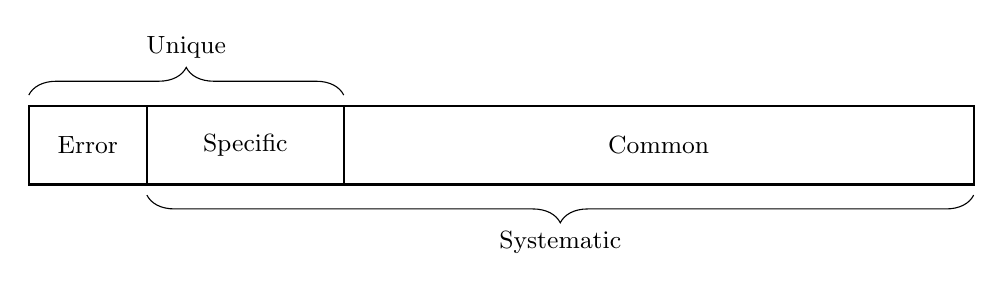
\begin{tikzpicture}
\draw[thick] (0,0) rectangle (1.5,1);
\node at (0.75,0.5) {\small{Error}};
\draw[thick] (1.5,0) rectangle (4,1);
\node at (2.75,0.5) {\small{Specific}};
\draw[thick] (4,0) rectangle (12,1);
\node at (8,0.5) {\small{Common}};
\draw [decorate,decoration={brace,amplitude=10pt,mirror},xshift=0pt,yshift=-1pt]
(1.5,-0.1) -- (12,-0.1) node [black,midway,yshift=-0.6cm] {\small{Systematic}};
\draw [decorate,decoration={brace,amplitude=10pt},xshift=0pt,yshift=1pt]
(0,1.1) -- (4,1.1) node [black,midway,yshift=0.6cm] {\small{Unique}};
\end{tikzpicture}

\end{document}